\begin{figure}[h]
\centering
\subfloat[CP]{
\fbox{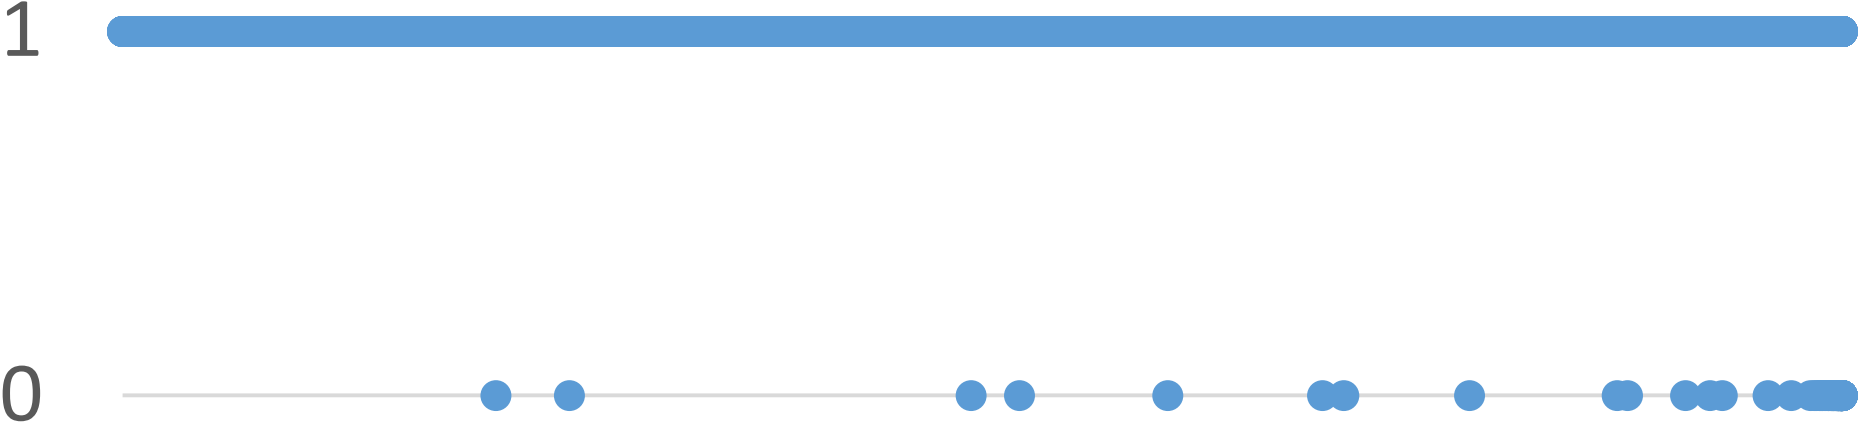
\includegraphics[width=0.22\linewidth]{figures/loop-cp.png}}
\label{fig:loop-cp}
}
\subfloat[CSD]{
\fbox{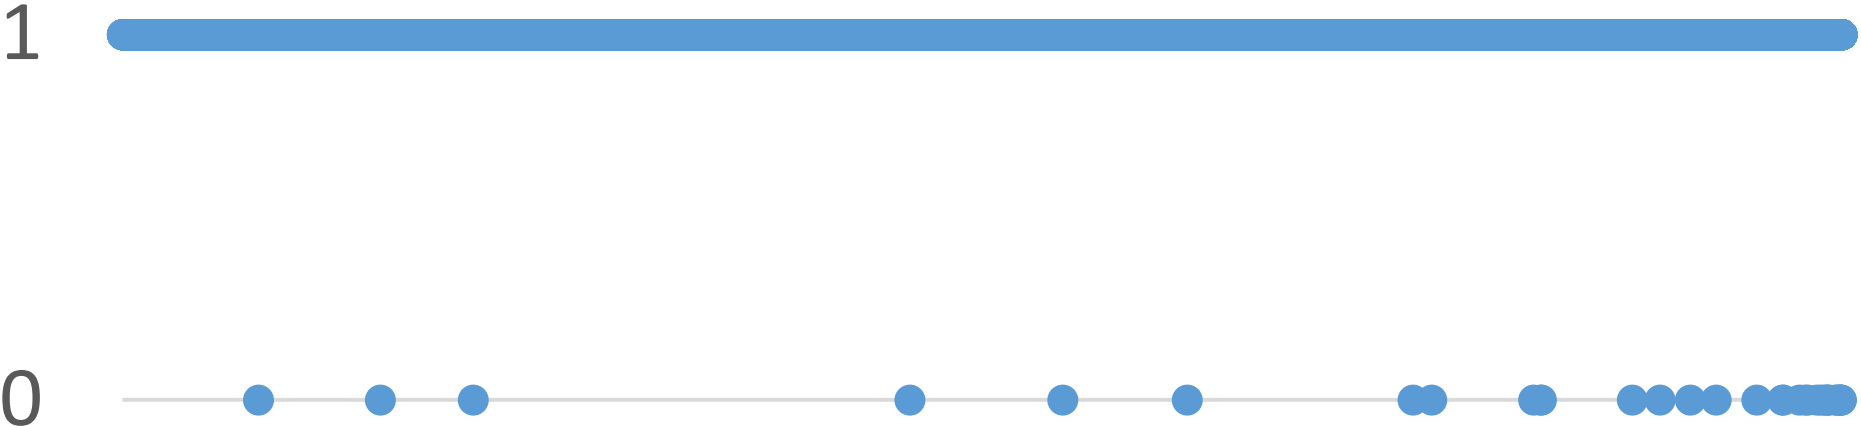
\includegraphics[width=0.22\linewidth]{figures/loop-csd.png}}
\label{fig:loop-csd}
}
\subfloat[DC]{
\fbox{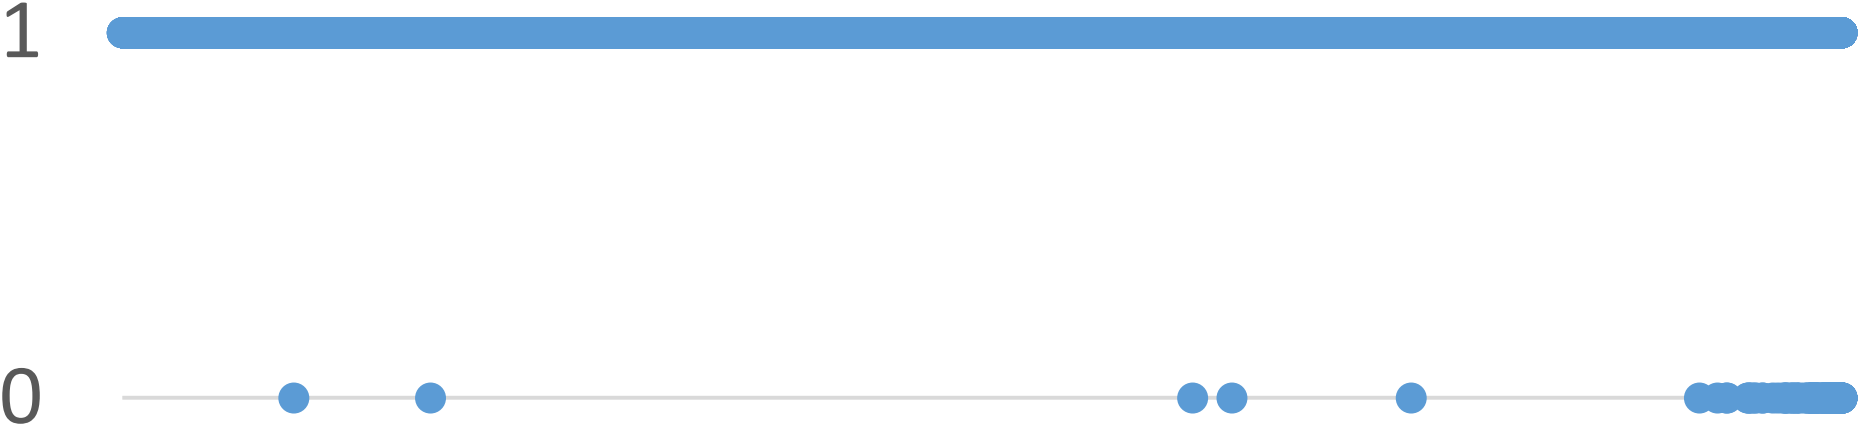
\includegraphics[width=0.22\linewidth]{figures/loop-dc.png}}
\label{fig:loop-dc}
}
\subfloat[LIC]{
\fbox{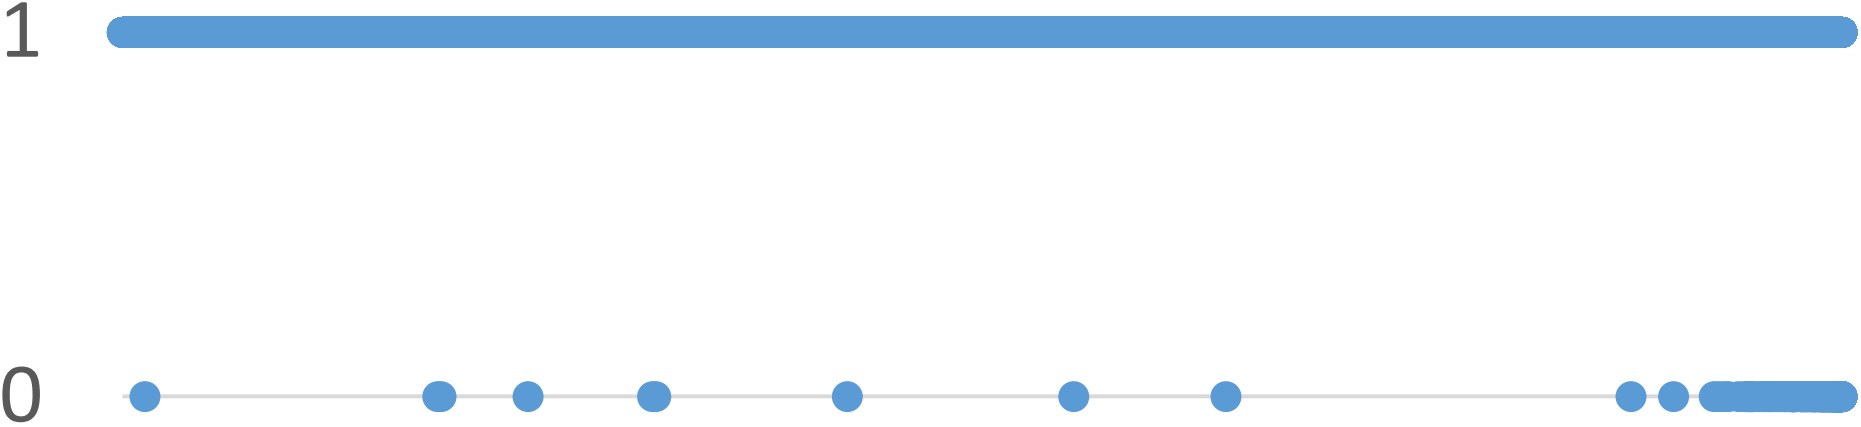
\includegraphics[width=0.22\linewidth]{figures/loop-lic.png}}
\label{fig:loop-lic}
}\\
\subfloat[USA]{
\fbox{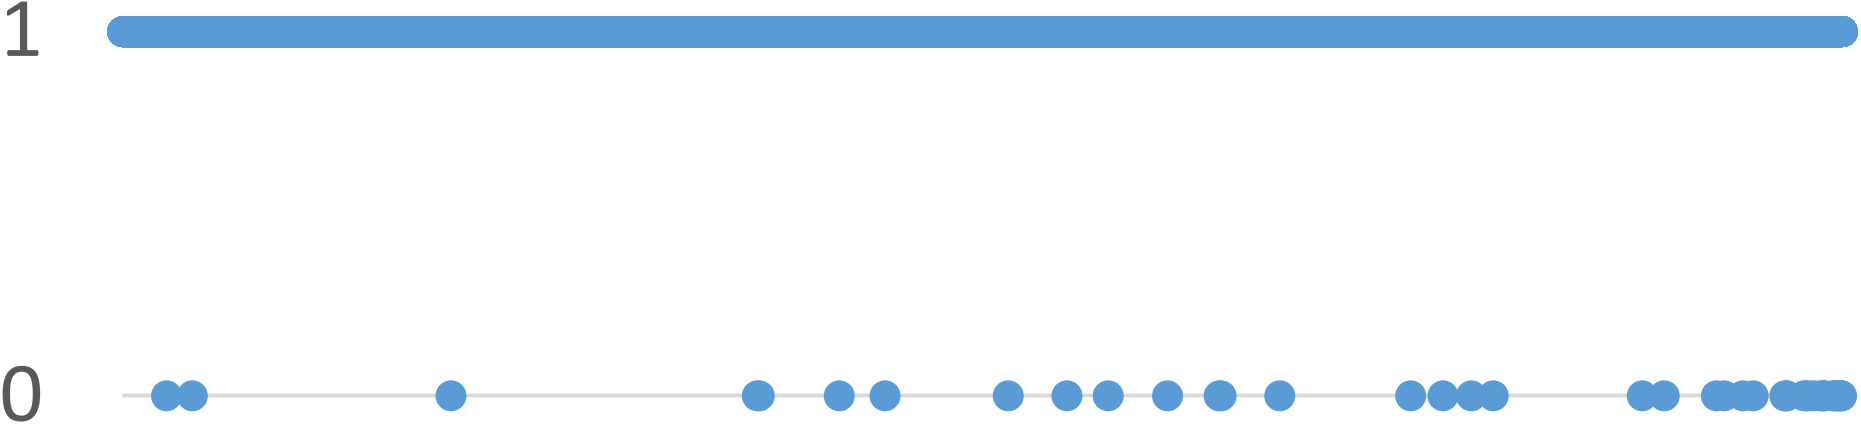
\includegraphics[width=0.22\linewidth]{figures/loop-usa.png}}
\label{fig:loop-use}
}
\subfloat[VFR]{
	\fbox{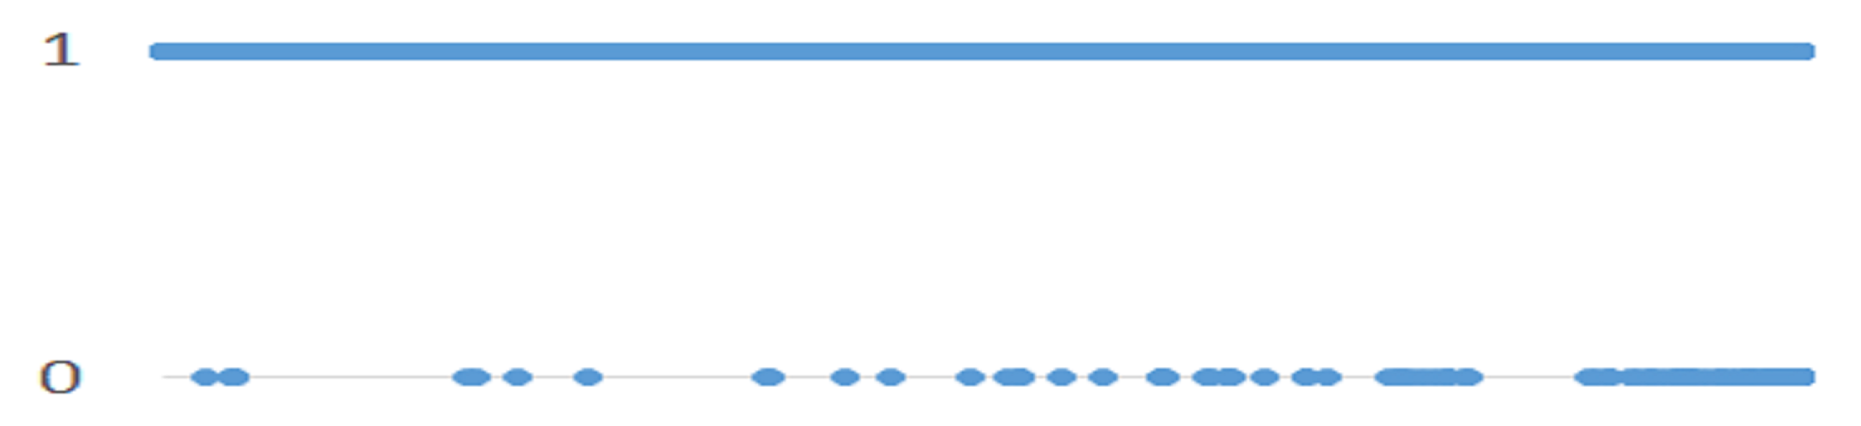
\includegraphics[width=0.22\linewidth]{figures/loop-vfr.png}}
	\label{fig:loop-vfr}
}
\subfloat[MWN]{
	\fbox{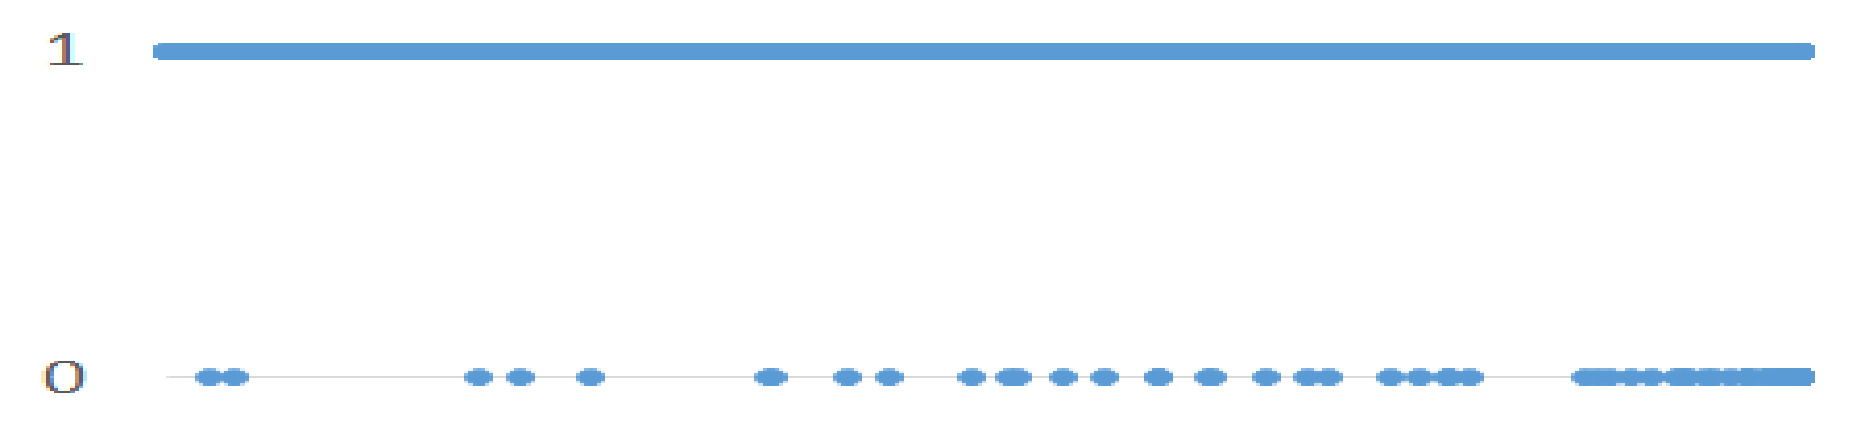
\includegraphics[width=0.22\linewidth]{figures/loop-mwn.png}}
	\label{fig:loop-mwn}
}
\subfloat[AE]{
\fbox{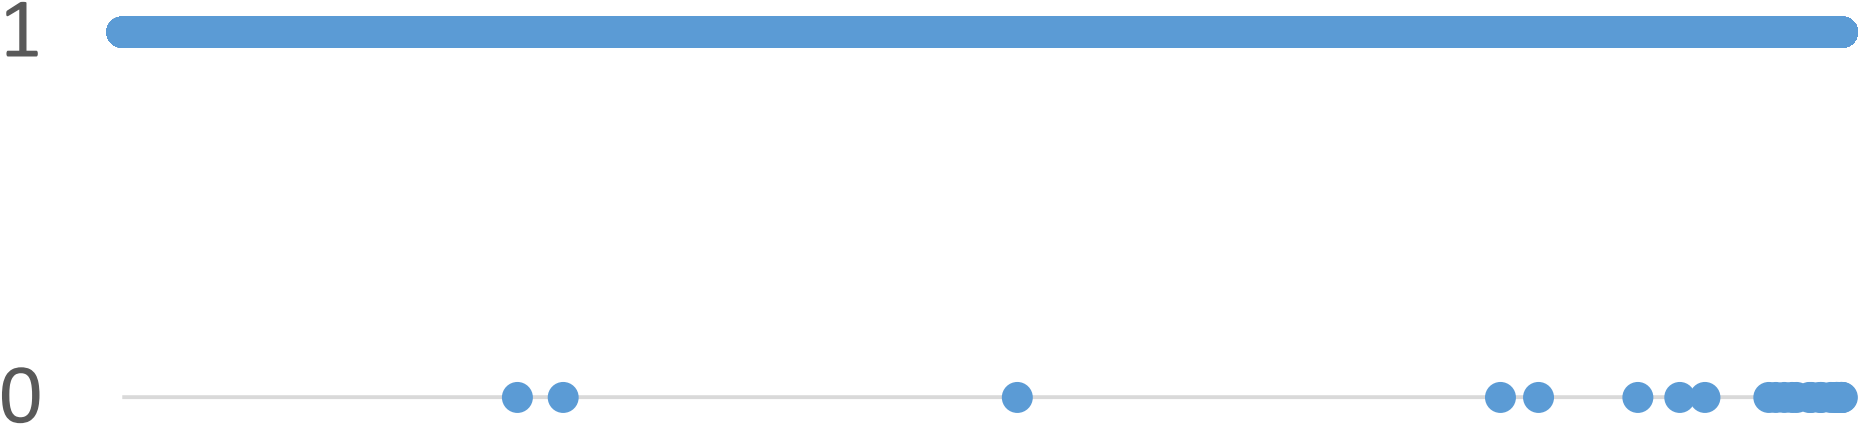
\includegraphics[width=0.22\linewidth]{figures/loop-ae.png}}
\label{fig:loop-ae}
}\\
\subfloat[LMA]{
\fbox{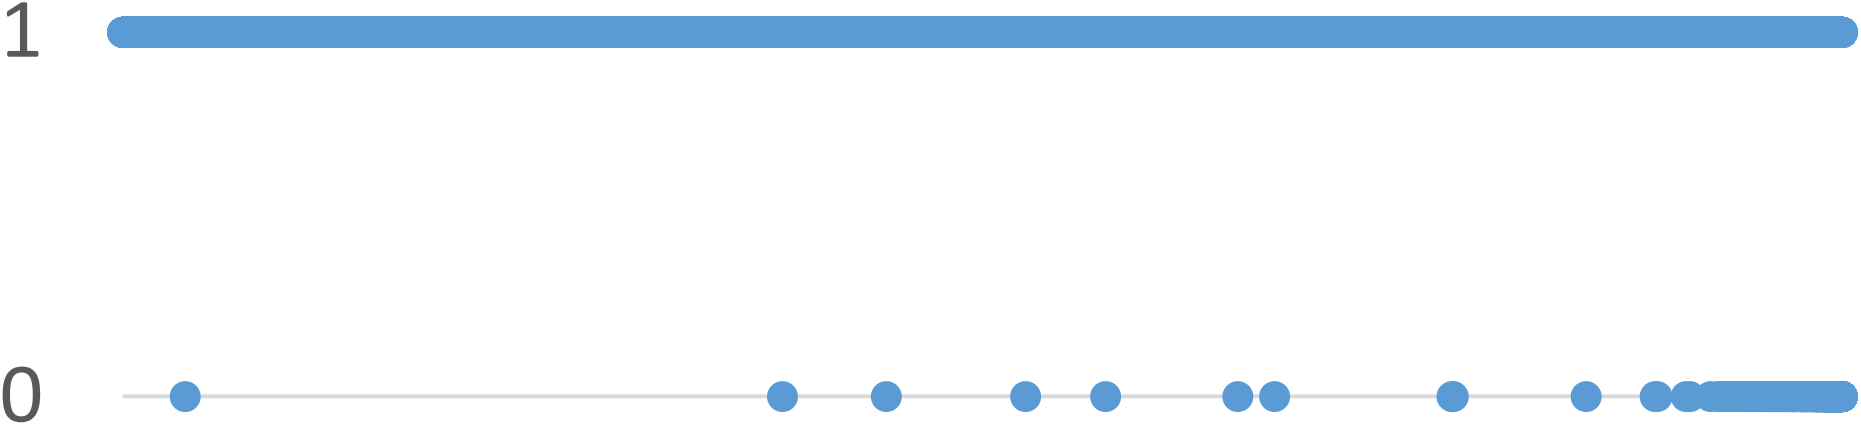
\includegraphics[width=0.22\linewidth]{figures/loop-lma.png}}
\label{fig:loop-lma}
}
\subfloat[LMNA]{
\fbox{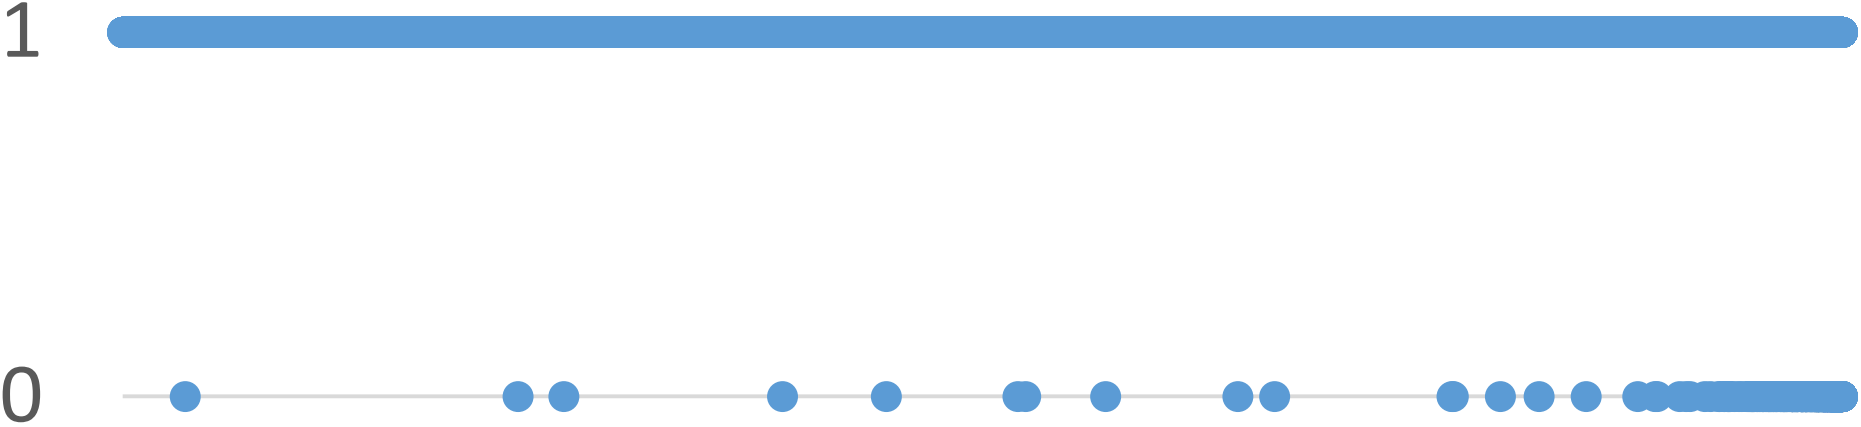
\includegraphics[width=0.22\linewidth]{figures/loop-lmna.png}}
\label{fig:loop-lmna}
}
\subfloat[LV]{
\fbox{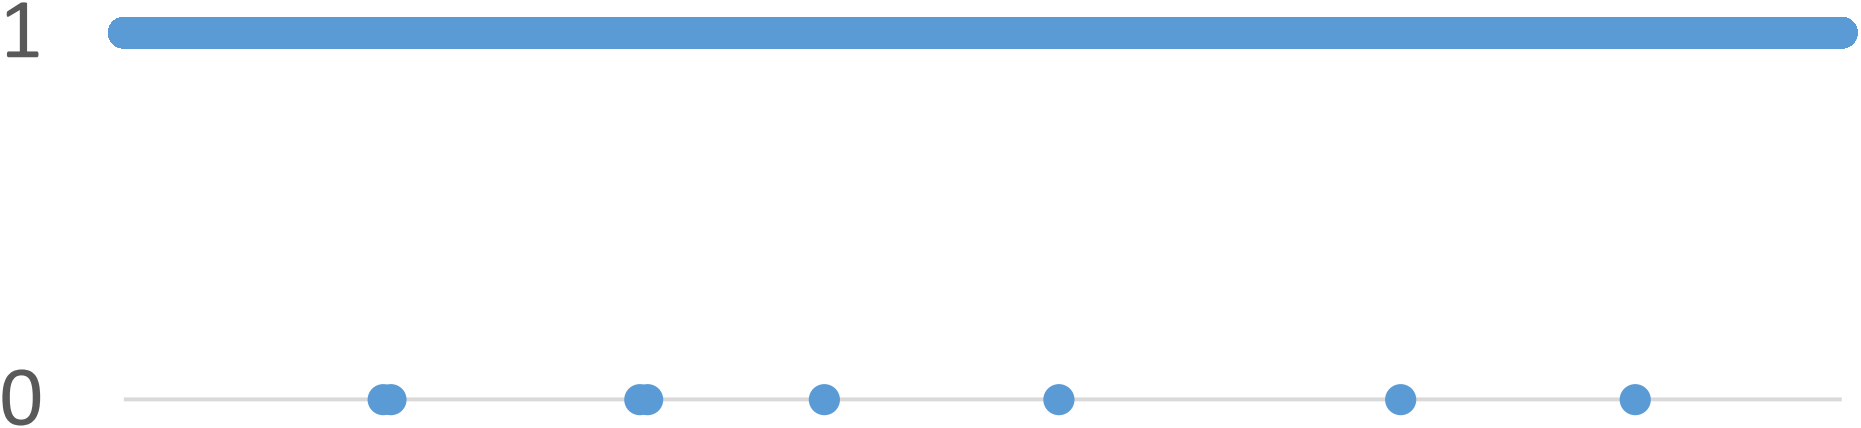
\includegraphics[width=0.22\linewidth]{figures/loop-lv.png}}
\label{fig:loop-lv}
}
\subfloat[NA]{
\fbox{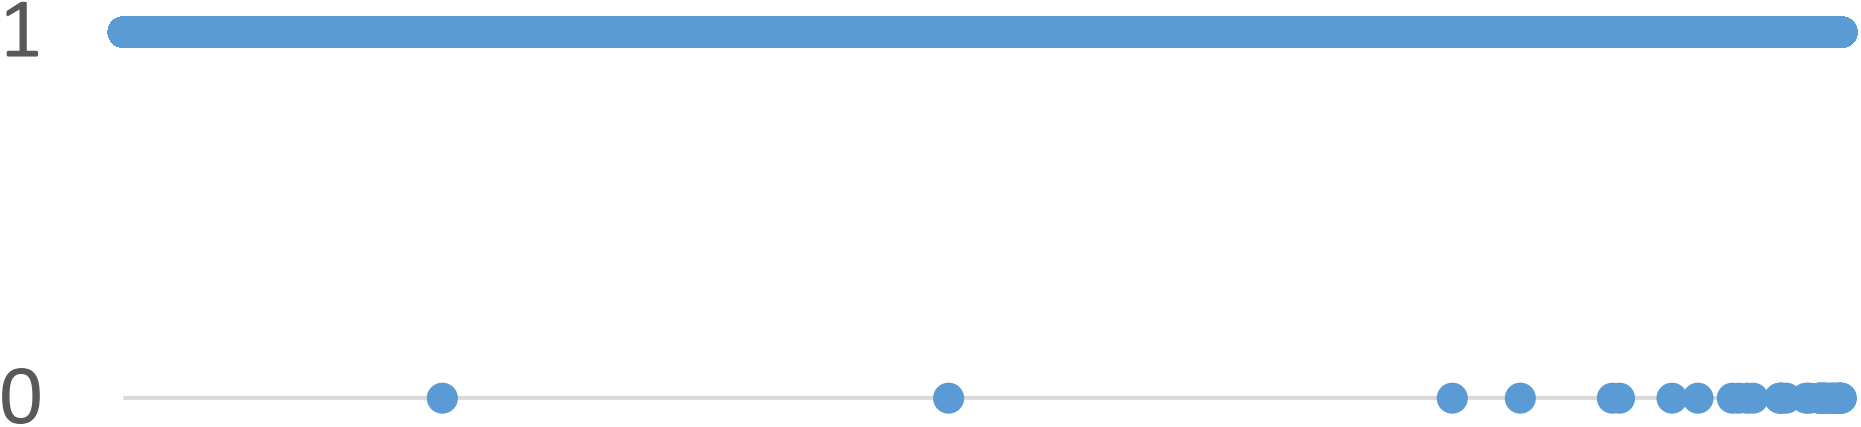
\includegraphics[width=0.22\linewidth]{figures/loop-na.png}}
\label{fig:loop-na}
}\\
\subfloat[RD]{
\fbox{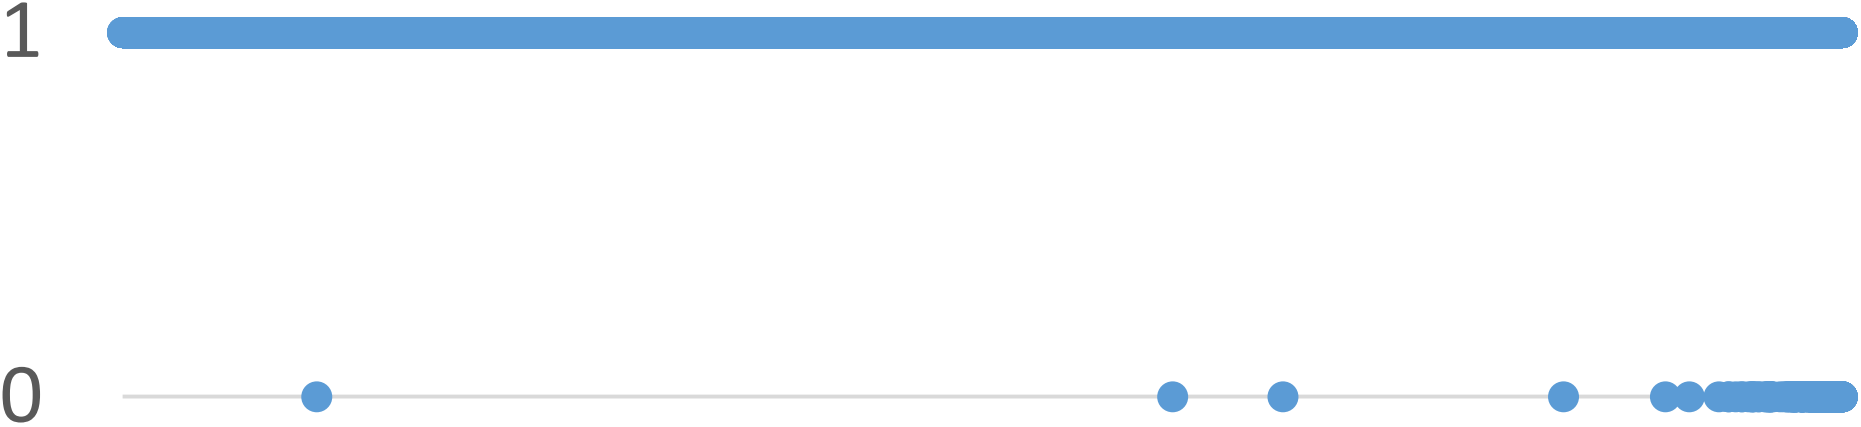
\includegraphics[width=0.22\linewidth]{figures/loop-rd.png}}
\label{fig:loop-rd}
}
\subfloat[RS]{
\fbox{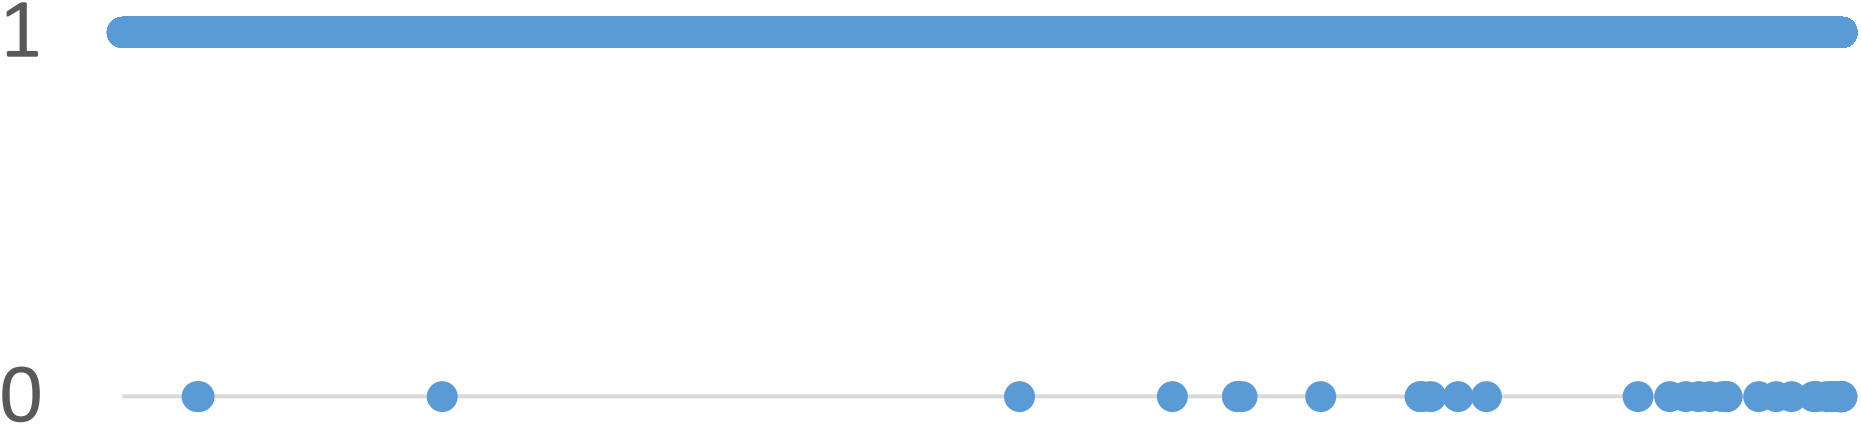
\includegraphics[width=0.22\linewidth]{figures/loop-rs.png}}
\label{fig:loop-rs}
}
\subfloat[VBE]{
\fbox{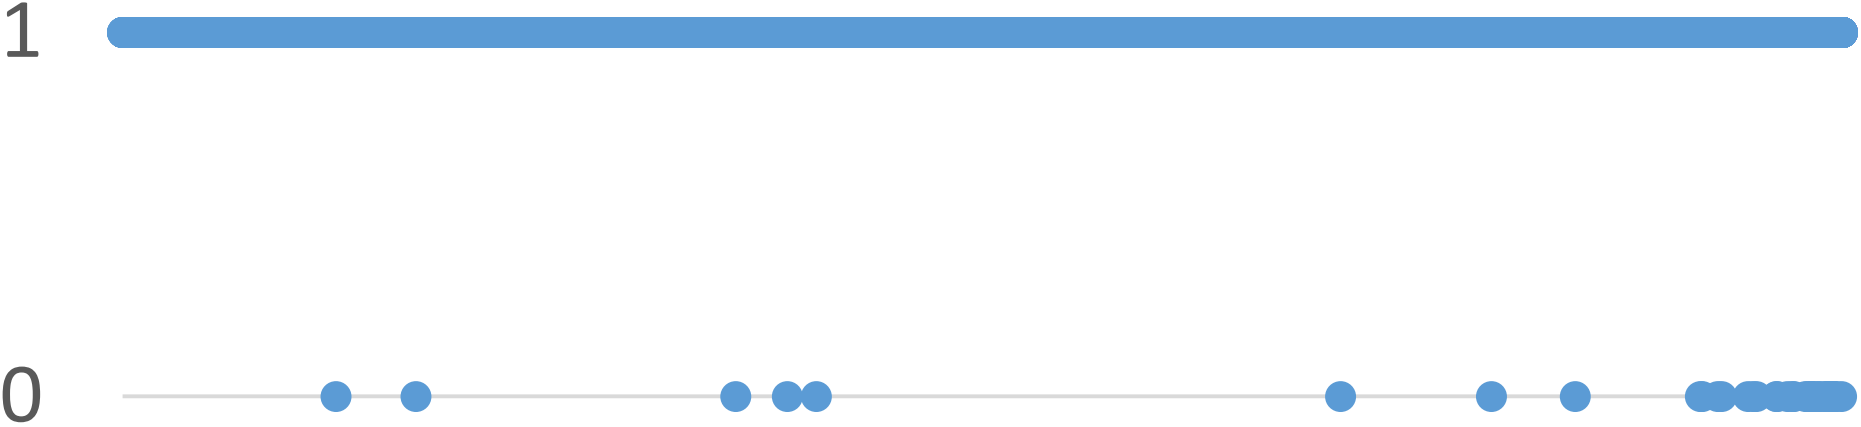
\includegraphics[width=0.22\linewidth]{figures/loop-vbe.png}}
\label{fig:loop-vbe}
}
\subfloat[SS]{
	\fbox{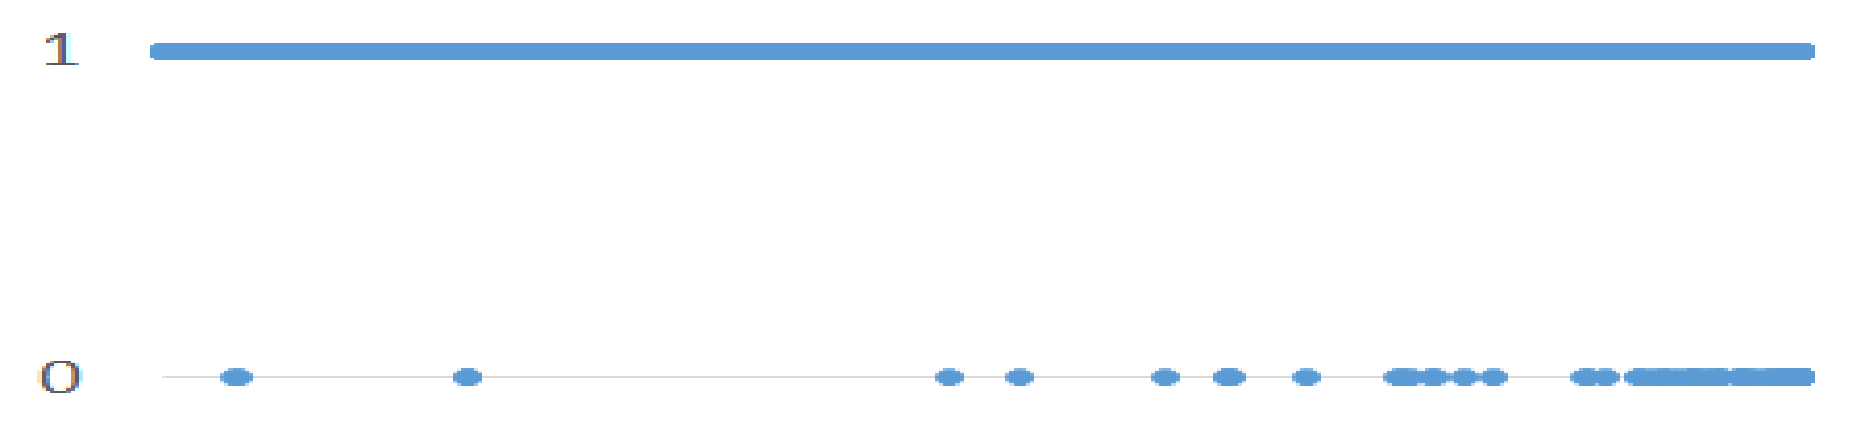
\includegraphics[width=0.22\linewidth]{figures/loop-ss.png}}
	\label{fig:loop-ss}
}\\
\caption{Scatter charts for analyses that have loop sensitive traversals. 
%$x$-axis lists the CFGs in the increasing of the node size. 
}
\label{fig:loops}
\end{figure}

